% \Image{Capa do livro (; )}{PNLD2022-005-01.png}
% \Image{Ilustração do livro (Ayllon/Lalau e Laurabeatriz; Ayllon)}{PNLD2022-005-04.png}
% \Image{Ilustração do livro (Ayllon/Lalau e Laurabeatriz; Ayllon)}{PNLD2022-005-05.png}
% \Image{Ilustração do livro (Ayllon/Lalau e Laurabeatriz; Ayllon)}{PNLD2022-005-06.png}



\documentclass[11pt]{extarticle}
\usepackage{manualdoprofessor}
\usepackage{fichatecnica}
\usepackage{lipsum,media9}
\usepackage[justification=raggedright]{caption}
\usepackage[one]{bncc}
\usepackage[ayllon]{../edlab}
\usepackage{marginnote}
\usepackage{pdfpages}
\usepackage[printwatermark]{xwatermark}
%\newwatermark[pagex=2]{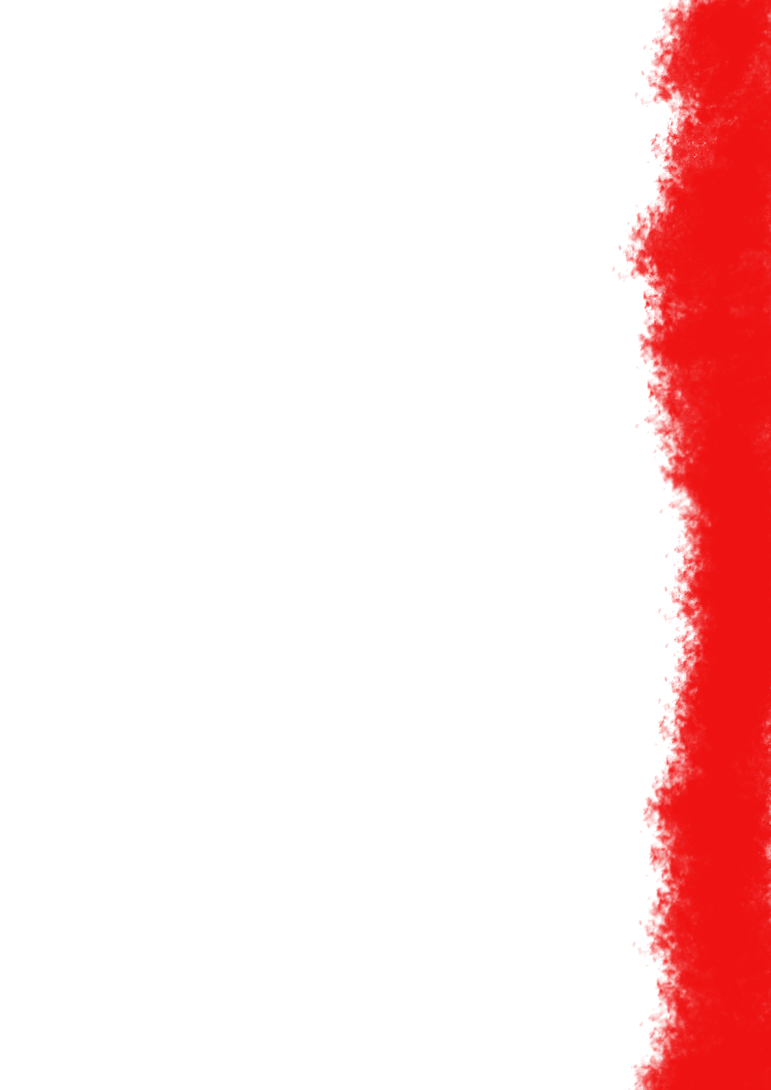
\includegraphics[scale=3.3]{watermarks/test-a.png}}	% página específica
%\newwatermark[oddpages]{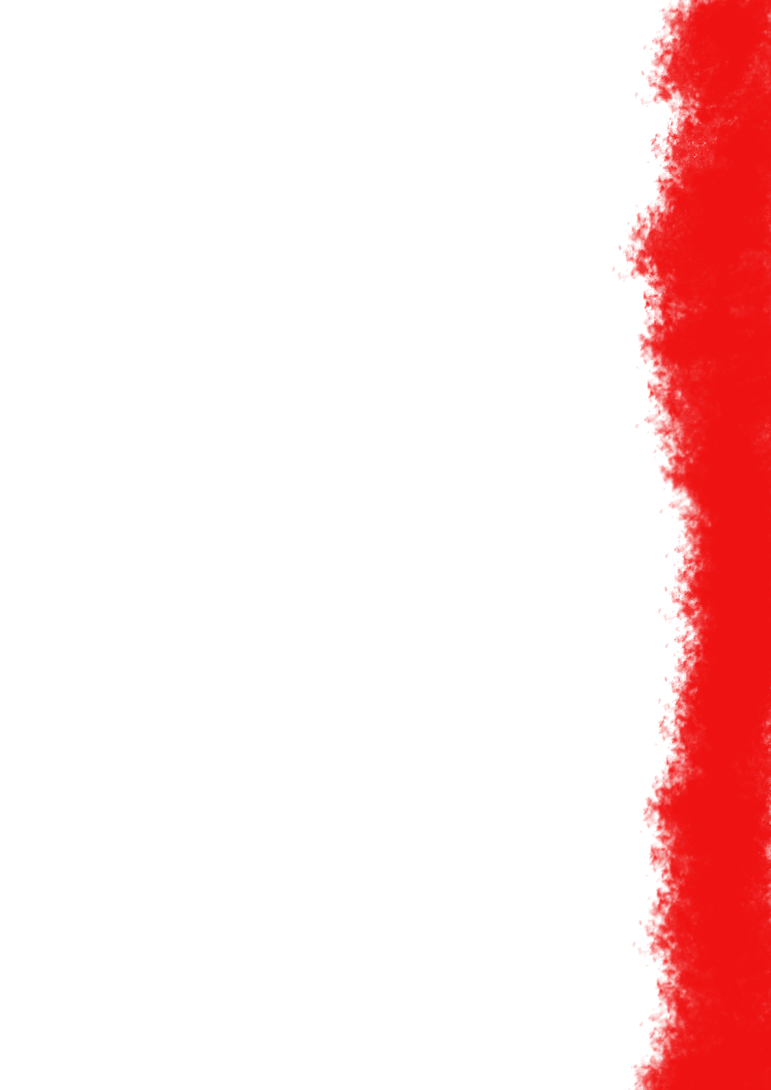
\includegraphics{watermarks/test-a.png}}			% páginas ímpars
%\newwatermark[evenpages]{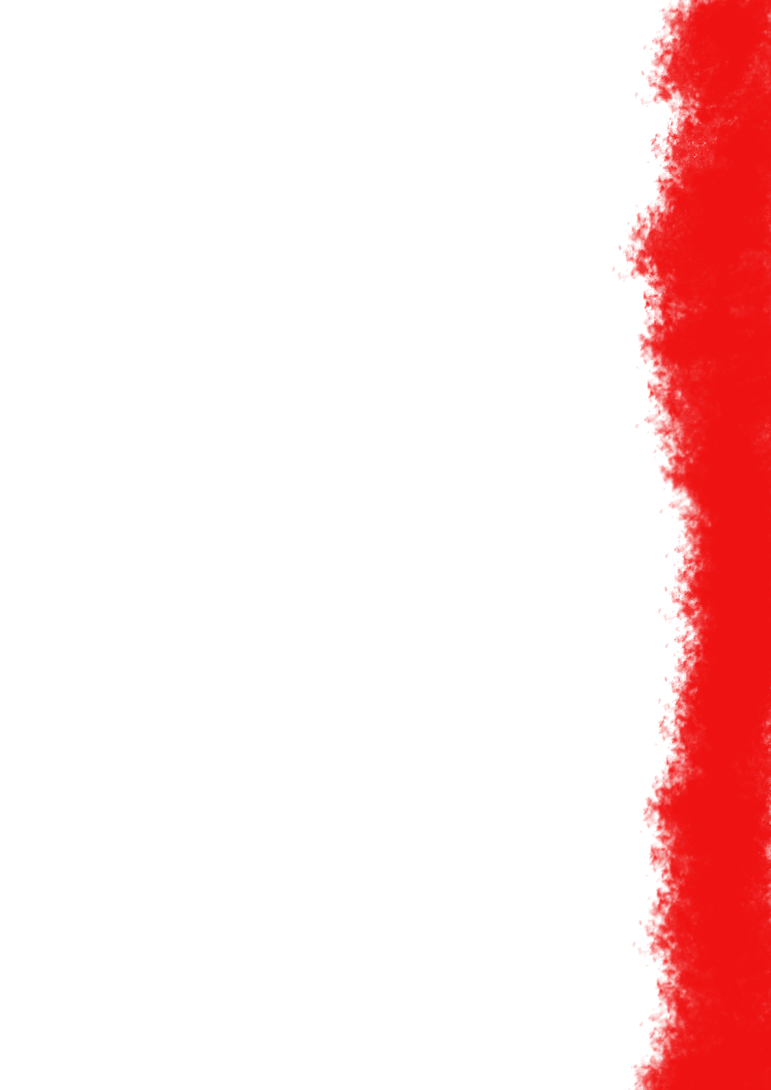
\includegraphics{watermarks/test-a.png}}			% págimas pares
\newwatermark[allpages]{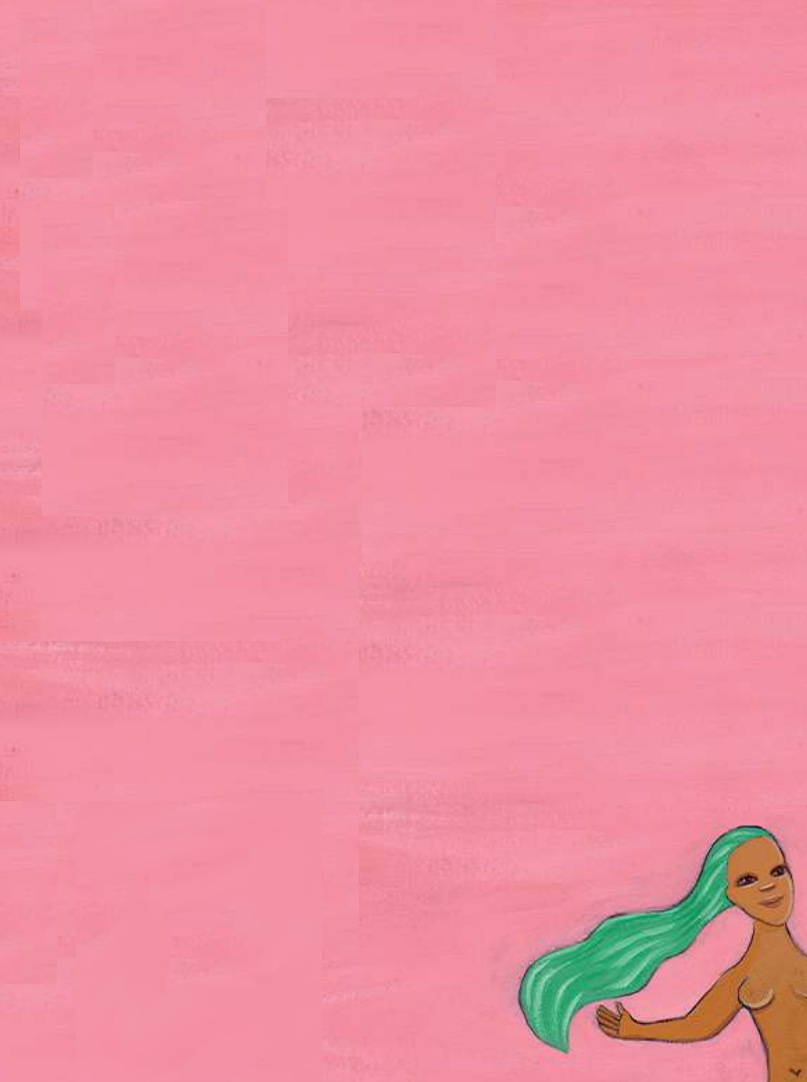
\includegraphics[scale=1]{watermarks/005.png}}

%\pagecolor{cyan!0!magenta!10!yellow!28!black!28!}

\newcommand{\AutorLivro}{Lalau e Laurabeatriz}
\newcommand{\TituloLivro}{As letras}
\newcommand{\Tema}{Quotidiano de crianças nas escolas; nas famílias e nas comunidades (urbanas e rurais)}
\newcommand{\Genero}{Poemas; trava-línguas; parlendas; adivinhas; provérbios; quadrinhas; etc}
\newcommand{\imagemCapa}{./images/PNLD2022-005-01.png}
\newcommand{\issnppub}{978-65-99430-45-9}
\newcommand{\issnepub}{978-65-99430-46-6}
% \newcommand{\fichacatalografica}{PNLD0001-00.png}
\newcommand{\colaborador}{{Paulo Pompermaier e Renier Silva}}

\begin{document}

\title{\TituloLivro}
\author{\AutorLivro}
\def\authornotes{\colaborador}

\date{}
\maketitle

%\begin{abstract}\addcontentsline{toc}{section}{Carta ao professor}
%\pagebreak

\tableofcontents



\section{Sobre o livro}

%550 caracteres
\paragraph{O livro} \textit{As letras}, de Lalau e Laurabeatriz, é uma viagem com o alfabeto através do Brasil. À cada página, o leitor é apresentado a uma letra do alfabeto, acompanhada de um pequeno poema e ilustrações de elementos da cultura, fauna e flora brasileir que começam com a letra indicada.
A forma como o alfabeto é abordado no livro aproxima as crianças das letras e da gramática básica ao relacionar o alfabeto a um universo afetivo, sensorial e lúdico.
Ao recorrer à poesia e a diferentes elementos da cultura brasileira (animais, ritmos musicais, lendas, frutas, instrumentos, alimentos, cores etc.), a obra permite o trabalho em diferentes esferas, explorando a imaginação da criança de inúmeras maneiras enquanto adquire e/ou consolida sua apreensão do alfabeto.


%822 caracteres
\paragraph{Descrição} Cada página do livro é dedicada a uma letra do alfabeto, trazendo poemas e ilustrações que reforçam a letra em questão, sequencialmente do A ao Z.
Para cada letra, um animal da fauna brasileira, uma lenda do folclore ou um traço cultural brasileiro será o protagonista: a arara, o bem-te-vi, o jacaré, a festa indígena Kuarup, o Uirapuru, o cacto xiquexique ou a sereia Yara. Apesar de o poema denominar apenas uma das figuras que ilustram a letra, o nome de todas as demais figuras começa com a letra em questão. No L, por exemplo, temos o poema: ``Onde a letra L / descobriu o lobo-guará? / na cor laranja / ou na luz do luar?''. Na página do L, além da ilustração do lobo-guará, encontramos a lula, o lambari e a libélula, possibilitando que o jovem leitor vá descobrindo esses animais enquanto aprende a nomeá-los e reconhecê-los.

A passagem pelo alfabeto, assim, se faz em paralelo à palavra rimada, à associação com as ilustrações da obra e ao contato com diferentes elementos da fauna, flora e cultura brasileira. Cria-se, assim, a possibilidade de perceber as letras de diferentes formas, construindo narrativas, rimas e canções em torno dos elementos mobilizados pela leitura. Ao final de toda página par, há um pequeno quadro com todas as letras do alfabeto, facilitando a memorização da ordem das letras e permitindo que se acompanhe o desenvolver de uma letra a outra.

%411 caracteres
\paragraph{Competências}
O livro \textit{As letras} trabalha a aquisição do alfabeto da língua portuguesa por meio de ilustrações para cada letra e pela palavra ritmada no poema. Mobiliza, assim, a aprendizagem dos alfabeto e da ordem das letras com base na competência de observar imagens, reconhecer os elementos ilustrativos e perceber a cadência de uma letra a outra.

Como esse processo se dá em paralelo com a apresentação de elementos culturais e tradicionais brasileiros, o livro contribui para expandir o repertório da criança, desde o vocabulário até a apreensão dos diferentes elementos que caracterizam e constituem as regiões brasileiras. Uma ótima maneira, portanto, de trabalhar também a alfabetização e apresentar à criança a diversidade que constitui o Brasil.

\reversemarginpar
\marginparwidth=5cm

\marginnote{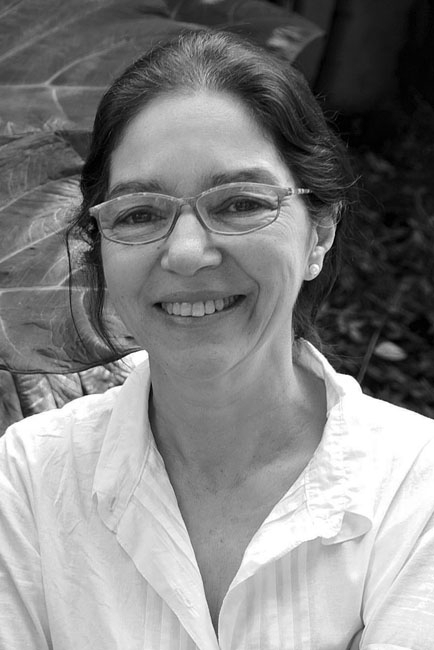
\includegraphics[width=\marginparwidth]{./images/PNLD2022-005-03.png}\\
A ilustradora Laurabeatriz (Arquivo pessoal)}

%862 caracteres
\paragraph{Aprofundamento} Este material tem a 
intenção de contribuir para que você consiga desenvolver um trabalho aprofundado 
com esta obra na sala de aula. Você encontrará informações sobre a autora, sobre 
o gênero e sobre os temas trabalhados ao longo do livro. Apresentaremos também 
algumas propostas de trabalho para a sala de aula que você poderá explorar livremente, 
da forma que considerar mais apropriada para os seus estudantes. Para a prática 
da Literacia Familiar, oferecemos um guia que pode ajudar nas orientações aos 
responsáveis pela criança, para incentivar o gosto pela leitura e contribuir para 
que os estudantes desenvolvam em casa habilidades que serão importantes no momento 
da alfabetização. Por fim, você encontrará sugestões de livros, artigos e sites 
selecionados para enriquecer a sua experiência de leitura e, 
consequentemente, a de seus estudantes.



\section{Sobre os autores}


%532 caracteres
\paragraph{A autora} Laurabeatriz, nome artístico de Laura Beatriz de Oliveira Leite de Almeida, nasceu no Rio de Janeiro em 1949, mas adotou São Paulo com sua cidade. Artista plástica apaixonada pela natureza, trabalha com desenhos, xilogravuras e pinturas, com as quais já participou de diversas exposições. Foi redatora publicitária e crítica de cinema do jornal \textit{Folha da Tarde}, além de ilustradora de outros jornais e revistas.

\paragraph{O autor} Lalau, nome artístico de Lázaro Simões Neto, nasceu em São Paulo, no bairro do Cambuci, em 1954. Formado em Comunicação Social, trabalhou com criação publicitária e projetos literários. Desde 1994 escreve poemas para crianças, incentivado pelo grande poeta José Paulo Paes.

\marginnote{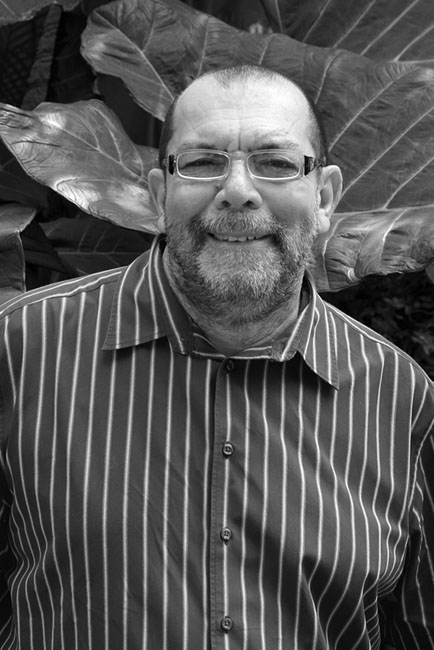
\includegraphics[width=\marginparwidth]{./images/PNLD2022-005-02.png}\\
O autor Lalau (Arquivo pessoal)}

%313 caracteres
\paragraph{Publicações} Além de \textit{Os números}, Lalau e Laurabeatriz já publicaram mais de 60 livros para crianças juntos. Desde 1994, quando publicaram seu primeiro livro juntos, \textit{Bem-te-vi e outras poesias}, não pararam mais de produzir, com Lalau escrevendo versos e Laurabeatriz ilustrando as histórias. Uma característica de todas as suas obras é a exploração da fauna e da flora brasileiras. No início dos anos 2000, publicaram a série ``Brasileirinhos'', com cinco volumes explorando a vida de ``brasileirinhos'' de diferentes regiões do país. 

%358 caracteres
\paragraph{Currículo} Lalau e Laurabeatriz já ganharam diversos prêmios por seus livros infantis. Em 1995, seu livro \textit{Fora da gaiola e outras poesias} recebeu o Prêmio \textsc{fnlij} de Melhor Livro de Poesia. Em 1997, \textit{Uma cor, duas cores, todas elas} recebeu o Título Altamente Recomendável pela Fundação Nacional do Livro Infantil e Juvenil (\textsc{fnlij}). A mesma instituição concedeu-lhes, em 1998, o prêmio de Melhor Livro Informativo por \textit{Histórias da preta}. Inaugurando a coleção Bicho-Poema, o livro \textit{Boniteza Silvestre} foi considerado um dos 30 melhores títulos infantis publicados em 2007 pela revista \textit{Crescer}. 
 


\section{Sobre o gênero}

%55 caracteres
\paragraph{O gênero} O gênero deste livro é \textit{poesia}. 


%596 caracteres
\paragraph{Descrição} Um dos meios mais expressivos de comunicação e inovação da linguagem, a poesia é uma das mais antigas formas de arte literária, anterior até mesmo à escrita, pois existe desde a tradição oral. Ela combina palavras, significados, sonoridades, ritmos e, muitas vezes, também imagens para permitir uma experiência estética. A linguagem poética é condensada e emotiva e busca trabalhar a língua de forma que o leitor experimente as palavras de uma forma nova. Na maior parte das vezes, a poesia é dividida em versos que, juntos, são chamados de estrofes. O ponto de vista do autor e sua visão pessoal do mundo estão muito presentes nesse tipo de texto e, justamente por essa particularidade, a experiência da leitura de uma poesia é extremamente individual e subjetiva.

%603 caracteres
\paragraph{Interação} Esse gênero é um grande aliado na formação do leitor. O olhar da criança para o mundo é, em essência, um olhar poético, calcado na curiosidade pelo mundo. A poesia é a forma perfeita de valorizar esse olhar e incentivar que a criança brinque com as palavras, observe os sons e experimente novos ritmos. Por sua liberdade e criatividade, a poesia tem potencial para estabelecer um diálogo único com os pequenos leitores. A presença de fantasias, imagens, repetição e símbolos permite uma maior identificação, pois a criança ainda está construindo seu mundo interior e experimenta a vida de forma diferente do adulto. 

\marginnote{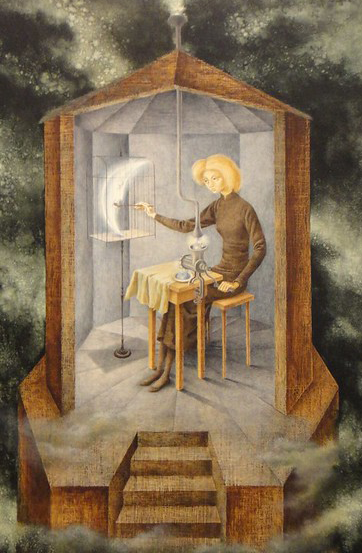
\includegraphics[width=\marginparwidth]{./images/PNLD2022-005-07.png}\\
O gênero poético incentiva a curiosidade e a imaginação. (LACMA/Remedios Varo; CC BY-NC 2.0)}

%862 caracteres
\paragraph{Competências} 
O caráter polissêmico do texto poético pode e deve ser explorado no ambiente escolar, assim como a dimensão lúdica da linguagem e as suas possibilidades. A própria estrutura do poema já produz aprendizado: ela seduz e desafia o leitor, apresenta ritmos, efeitos sonoros e, ao mesmo tempo, apresenta novas vivências, oferecendo possibilidades para a criança simbolizar suas próprias experiências. Cada dupla de páginas do livro \textit{As letras} apresenta um poema, a letra do alfabeto em evidência e ilustrações cujos nomes começam com a referida letra. Assim, a apreensão do alfabeto se faz em paralelo com a descoberta das ilustrações e dos elementos abordados no poema. A leitura do poema, realizada pelo educador, aumenta o repertório do aluno, incentiva o desenvolvimento do vocabulário e da fluidez do discurso.
A associação entre a aprendizagem do sistema alfabético e a poesia, ademais, permite explorar múltiplas competências ao mesmo tempo, pois relaciona os princípios do alfabeto à linguagem poética, introduzindo o aluno no universo lúdico e artístico da poesia.



\section{Temas}

\subsection{Quotidiano de crianças nas escolas; nas famílias e nas comunidades (urbanas e rurais)}

%136 caracteres
\paragraph{Abordagem} As letras são as protagonistas desta história. 
Todos os poemas acompanham a passagem pelo alfabeto, do A ao Z, familiarizando as crianças com o sistema alfabético que perpassa o cotidiano escolar, familiar e social.

%206 caracteres
\paragraph{Descrição} O livro oferece uma ótima oportunidade de explorar 
e aprofundar o sistema do alfabeto com as crianças, além de abrir espaço para o diálogo com a poesia e os demais elementos da fauna e flora brasileira que ilustram as letras.

%275 caracteres
\paragraph{Competências} Este tema relaciona-se, principalmente, ao 
campo da experiência Espaços, tempos, quantidades, relações e transformações 
descrito pela \textsc{bncc}, que explora a curiosidade infantil sobre o mundo 
para proporcionar a construção de conhecimento a partir da observação e exploração.

\subsection{Animais da fauna local, nacional e mundial}

%136 caracteres
\paragraph{Abordagem} Os animais também são fundamentais nesse livro. 
Todos os poemas do livro trazem nomes e ilustrações de animais das diferentes faunas brasileiras.

%206 caracteres
\paragraph{Descrição} O livro oferece uma ótima oportunidade de explorar 
as características destes animais com as crianças, além de abrir espaço para uma 
conversa sobre outros animais que façam parte do repertório dos estudantes. 

%275 caracteres
\paragraph{Competências} Este tema relaciona-se, principalmente, ao 
campo da experiência O eu, o outro e o nós 
descrito pela \textsc{bncc}, pois explora, a partir de elementos de diferentes biomas, as diferenças que constituem o Outro, as particularidades formadoras do eu, e os elementos comuns, em meio à diversidade, que possibilitam a existência de um nós.



\section{Modelagem de aula}
A seguir você encontrará a descrição de uma aula modelo como exemplo 
prático de exploração do livro com estudantes. Esta seção apresentará 
orientações sobre como organizar a sala de aula para receber os 
estudantes, exercitar a interação verbal e prepará-los para o 
momento da leitura.

Em seguida, você encontrará a \textbf{Leitura dialogada}, um 
tópico destinado a te orientar para o momento específico da 
leitura com os estudantes. Por fim, no tópico 
\textbf{Propostas de atividades}, você encontrará ideias 
de práticas que pode explorar com as crianças em sala de 
aula antes, após e durante a leitura. 

Essas atividades podem ser trabalhadas de acordo com a 
disponibilidade do seu cronograma. Fique à vontade para adaptá-las 
da forma que achar melhor para os seus estudantes. Cada turma é única 
e o seu conhecimento prático das características de cada aluno será 
essencial para definir a melhor forma de aplicar essas ideias. 

O objetivo deste manual é oferecer algumas ideias 
e inspirações para um trabalho que pode ser desenvolvido tanto 
a curto, quanto a médio e longo prazo. Sinta-se à vontade para 
personalizar a aula e torná-la sua, aplicando seus conhecimentos, sua 
personalidade e aproveite para fortalecer 
seu vínculo com a turma.


\subsection{Antes de ler}

\BNCC{EI03EO02}
\BNCC{EI03EO03}
\BNCC{EI03EO07}
\BNCC{EI03CG02}
\BNCC{EI03CG05}
\BNCC{EI03ET01}
\BNCC{EI03ET05}


%Alterar o nível escolar nesse parágrafo.
Como este trabalho será realizado com crianças da \textbf{Pré-escola}, 
que ainda não têm tanta intimidade com o livro enquanto objeto, você terá o 
papel essencial de mediar este contato. 

Nosso objetivo é que os próprios estudantes possam manusear 
e explorar o livro de forma autônoma, mas, para que isto aconteça, você 
pode ajudar a tornar o caminho mais convidativo com atividades que tenham 
intencionalidade educativa. 

A \textsc{bncc} define intencionalidade educativa como ``organização 
e proposição, pelo educador, de experiências que permitam às crianças 
conhecer a si e ao outro e de conhecer e compreender as relações com a 
natureza, com a cultura e com a produção científica, que se traduzem nas 
práticas de cuidados pessoais (alimentar-se, vestir-se, higienizar-se), 
nas brincadeiras, nas experimentações com materiais 
variados, na aproximação com a literatura e no encontro com as 
pessoas''.\footnote{\textsc{bncc}, página 39}

É importante manter essa intencionalidade em mente não apenas na condução 
das atividades propostas neste manual, mas também para aproveitar as 
oportunidades espontâneas de construir conhecimentos que podem surgir durante 
a interação direta com os estudantes.

\begin{enumerate}
%836 caracteres
\item \textbf{O ambiente}\quad Antes de iniciar o trabalho com o livro, é importante que você 
prepare o ambiente para receber a turma. Como o trabalho com o livro terá 
três momentos (antes, durante e depois da leitura), seria interessante que você 
criasse um ambiente para cada etapa. Nas \textbf{Sugestões de referências complementares} 
você encontrará um artigo que discorre sobre a importância da organização da sala 
de aula para a educação infantil, que pode ser um bom guia para a criação desses 
ambientes.
Para o momento antes da leitura, sugerimos uma atividade que estimulará a imaginação do aluno, a capacidade de resolver pequenos problemas e associação de letras e objetos. O professor deverá dividir cada letra do alfabeto entre os alunos e pedir para que tragam um objeto ou desenho de casa que corresponda à sua letra, definida por sorteio. Se houver mais de 26 alunos, ou menos, você pode distribuir as letras proporcionalmente. Os pais devem ser avisados antecipadamente para que se organizem, salientando aos responsáveis pela criança que a escolha do objeto seja realizada junto com o estudante. Pode ser realizada em sala de aula, biblioteca ou espaço aberto.

%413 caracteres
\item \textbf{Materiais}\quad Colagens, desenhos, objetos de casa, cores que começam com a letra sorteada.

%632 caracteres
\item \textbf{Desenvolvimento}\quad O professor dividirá as letras do alfabeto entre os alunos e solicitará a cada um que traga um objeto ou desenho de casa que corresponda à sua letra, definida por sorteio. Com a ajuda dos pais, as crianças pode trazer o que tiverem em casa que se enquadre na sua letra sorteada: colagens, desenhos, objetos de casa, cores que começam com a letra sorteada. O importante é estimular a imaginação do aluno e a capacidade de resolver pequenos problemas. É importante dialogar com os responsáveis para não escolherem pela criança, e sim facilitarem sua escolha. É imprescindível que os responsáveis participem do processo de ensino/aprendizagem de seus filhos, pois isso possibilita uma aquisição de conhecimento mais significativa e afetiva. No dia combinado, peça para que os alunos digam como foi o processo para encontrar o objeto com a letra sorteada. Proporcione uma conversa livre e descontraída, organizando os relatos um de cada vez.

\item \textbf{Perguntas para avaliar}\quad Como os alunos se comportaram diante do desafio proposto? A turma se engajou e se divertiu? Como se sentiram no processo de procura do objeto? A criança teve protagonismo na escolha? 

\end{enumerate}


\subsubsection{A interação verbal} 
Criar situações em que as crianças precisam dialogar diretamente com 
você é uma das práticas mais importantes de Literacia, pois elas estimulam 
o desenvolvimento linguístico, ampliam o vocabulário e reforçam a 
capacidade dos estudantes de compreenderem o que ouvem e se expressarem 
pela fala. O diálogo livre com a criança também reforça sua autoestima, pois 
a faz se sentir ouvida e valorizada pelo adulto, ao vê-lo prestar atenção 
no que ela tem a dizer. Portanto, sempre que possível, reserve um tempo na 
aula apenas para a interação verbal. 

Como esse tipo de interação é espontânea e intimamente atrelada ao 
desenvolvimento de cada estudante, nossas orientações não serão específicas. 
A ideia é que você adapte este momento de acordo com as respostas e os 
repertórios das crianças. É um momento de estreitamento de vínculos e, portanto, 
fique à vontade para ser espontânea e para explorar os tópicos que achar 
mais interessantes para a sua turma.

Inicie as conversas com naturalidade, seguindo os objetos de atenção das crianças. 
Você pode partir de objetos que estejam analisando
para iniciar um assunto e incentivar que se expressem. Ainda que a
criança não fale corretamente, continue interagindo, 
pois a intenção aqui é que a criança perceba que outras pessoas estão respondendo 
à sua comunicação. 

Fique atento a todas as formas de expressão: os gestos, as falas, as 
expressões faciais, para onde olham\ldots{} tudo pode ser explorado durante a conversa. 
Demonstre curiosidade sobre eles, seja um ouvinte entusiasmado e incentive que eles 
conversem entre si. Faça perguntas e construa a resposta junto com as crianças. 

A seguir, algumas dicas que podem contribuir para que a interação verbal 
seja produtiva em sua sala de aula: 

\begin{enumerate}
\item Sente-se no chão e brinque com eles, estabelecendo 
contato visual. Além das pequenas frases que conseguem formar, vocalizações, 
gestos e expressões faciais podem ser boas formas de comunicar.

\item Não se esqueça que a conversa é uma troca e, portanto, 
evite ficar falando sozinho ou desvalorizar as respostas das 
crianças quando não conseguem formular frases completamente articuladas. 
Nunca descarte uma tentativa de comunicação. 

\item Evite utilizar falas negativas que desencorajam o diálogo. 
Se precisar que a turma 
corrija algum comportamento, explique claramente a razão e 
oriente com calma. Incentive positivamente as crianças e 
destaque o motivo de seus elogios. 

\item Aproveite alguns momentos durante a conversa para chamar 
a atenção das crianças para os sons das palavras e das letras que você 
acabou de usar ou que eles pronunciaram.  

\item Explore possibilidades de interação como apontar e 
nomear objetos, pessoas e animais, imitar a criança ou pedir que 
ela o imite, fazer caretas, reproduzir sons de 
animais para que repitam, ensinar os nomes de partes do corpo, 
entre outras atitudes que estimulem a comunicação com a criança. 

\item Muitas dessas dicas poderão ser aproveitadas pela 
família durante a prática da Literacia Familiar. Portanto, 
se achar necessário, compartilhe algumas destas orientações 
com as famílias dos estudantes.
\end{enumerate}


\subsection{A leitura dialogada}
Este é o momento em que será realizada a leitura propriamente dita. 
Se possível, crie um \textit{cantinho da leitura} em sua sala de aula. Um 
ambiente confortável, de preferência em que todos se sentem no chão ou 
em pufes para que consigam enxergar as ilustrações do livro que está 
sendo lido e interagir com facilidade. Se houver possibilidade, mantenha 
sempre os livros da turma em uma altura da estante que permita fácil 
acesso para os estudantes ou guarde os livros em uma caixa que as crianças 
possam mexer com autonomia. É importante que elas tenham autonomia para 
acessar os livros e se sintam à vontade para pegá-los sempre que quiserem.

\Image{É importante que o cantinho da leitura proporcione autonomia para as crianças. (Elza Fiúza/ Agência Brasil; CC BY-NC 2.0)}{PNLD2022-005-08.png} 

Outra possibilidade de ambiente para esta leitura, se a escola permitir, 
é efetuar essa leitura ao ar livre, embaixo de uma árvore, onde as crianças 
possam ouvir os sons dos pássaros e sentir o cheiro da grama. Sair da sala 
de aula pode oferecer um ótimo leque de experiências aos seus estudantes e 
reforçar a conexão entre a natureza do livro e a realidade.  

Reserve uma boa parte da aula para o momento da leitura com os estudantes, 
pois é importante que esse momento aconteça sem pressa. O objetivo da 
leitura dialogada é que seja uma leitura em bate-papo. A criança deve 
assumir um papel ativo na leitura, mesmo que ainda não seja capaz de 
ler sozinha. Além de promover o gosto pela leitura, esta prática estimula 
o desenvolvimento da linguagem, enriquece o vocabulário e 
aumenta o conhecimento de mundo.

%Especificar o livro.
No caso de \textit{As letras} o diálogo durante a leitura é 
ainda mais importante, considerando que muitas palavras dos poemas são desconhecidas pelas crianças e, portanto, a compreensão do texto se apoiará principalmente na sua interação com as crianças. 
Você deve interagir com eles durante toda a 
leitura, fazendo perguntas e partindo de detalhes do livro para 
levantar novas questões. 

A seguir, algumas orientações para aproveitar este momento e desenvolver uma atividade durante a leitura: 

\begin{enumerate}
%177 caracteres
\item \textbf{Contexto}\quad Esta atividade parte da atividade antes da leitura sugerida anteriormente. Os alunos devem permanecer com as letras sorteadas, e o professor deve se organizar para que todos participem. É uma atividade que procura imprimir certa dinâmica à leitura, engajando os estudantes e convocando-os à participação. A ideia é proporcionar protagonismo e autonomia para as crianças, além de valorização pessoal e coletiva. Esta atividade trabalha a socialização, o desenvolvimento da linguagem, associação e simbolização. Pode ser realizada em sala de aula ou na biblioteca, apenas com o livro e um alfabeto impresso (ou escrito, com letras garrafais, em uma folha em branco).  


\item \textbf{Desenvolvimento}\quad Antes de iniciar a leitura dos poemas, explique para os alunos que cada um deles corresponde a uma letra do alfabeto, como na atividade anterior (os alunos continuarão com as mesmas letras). Quando for iniciar a leitura, o educador pode primeiramente convidar o aluno  que está com a letra correspondente para se juntar a ele na frente da sala. Quando for ler o poema referente ao A, por exemplo, chame a criança que está com a letra A para a leitura compartilhada, enquanto os outros alunos ficam sentados em suas cadeiras para aguardar sua vez de ir para a frente. Após o professor finalizar a leitura do poema, pedirá para o aluno tentar reconhecer as imagens que correspondem à sua letra e pedir que repita a pequena estrofe da página de sua letra. A atividade deve ser pensada de acordo com o nível de desenvolvimento de cada criança: algumas já podem tentar ler sozinhas, e é importante que se dê essa opção para quem você observa que pode fazê-lo. Após todos os alunos serem chamados, todas as letras do alfabeto terão sido lidas com seus poemas, dinamizando a leitura dialogada e associando, ao campo afetivo da sala e das relações entre os colegas, a ordem das letras do alfabeto.
 
%230 caracteres
\item \textbf{Manuseio}\quad Deixe que as crianças manuseiem o livro 
e explore com elas todos os elementos que o compõem. Mostre o que é a 
capa e onde estão as páginas.

%495 caracteres
\item \textbf{Diálogo}\quad Como cada poema vai ter a participação de um aluno, todos vão interagir no diálogo, e a própria forma da dinâmica possibilita que o conteúdo seja transmitido aos alunos, pois vão sendo chamados pelas letras correspondentes na ordem do alfabeto. Após a leitura, o aluno é convidado a repetir o que lembra do poema e interagir com as figuras e imagens que aparecem para sua letra, apontando quais identifica e quais desconhece. Se o aluno não souber ou não se sentir confortável a participar no seu momento, convide os colegas a colaborarem e ajudarem com suas opiniões.

%346 caracteres
\item \textbf{Escuta}\quad Elogie atitudes positivas, como 
a boa interação com o poema lido e a solicitação de interagirem com ele. Se os estudantes tentarem 
tomar o seu lugar e começar a falar sobre o poema, valorize e escute com atenção o que estiverem falando. Mas não 
force a leitura. Se as crianças estiverem cansadas, faça outra atividade 
e retorne depois. 

\includepdf[nup=2x3, 				% grid
			%offset=-15mm -5mm, 	% posição
			scale=.8, 				% tamanho da página
            delta=4mm 4mm, 			
            frame,
            pages={4-5,22-23,42-43}]{./pdfs/\jobname_MIOLO.pdf}

%935 caracteres
\item \textbf{Leitura}\quad Faça perguntas e comentários que aumentem o 
interesse e aticem a curiosidade das crianças sobre os poemas e as letras. Faça 
perguntas ou comentários como: 

\begin{itemize}
\item O que representa essa figura?
\item O que rima com a palavra final do poema?
\item A arara é vermelha e azul, voa pelos ares e mora nas florestas!
\end{itemize}

Não tenha pressa em passar as páginas. Deixe que os estudantes 
observem as ilustrações e o poema, dê tempo para que construam suas imagens 
mentais a partir do poema que foi lido e das ilustrações presentes na página. 

Ao explorar a leitura do poema, dê emoção 
à leitura. Enfatize as palavras desconhecidas, marque as rimas presentes nos versos,
capriche nas expressões faciais e traga, ao final, comentários sobre os animais ilustrados.
Deixe-se guiar pela atenção das crianças, mas se perceber que 
elas estão dispersas ou saltando aleatoriamente as páginas, ajude-as 
a retornar ao poema. Crie um ambiente amigável onde a criança 
se sinta à vontade para fazer perguntas e comentários durante a leitura.

%382 caracteres
\item \textbf{Interação}\quad Nomeie os elementos das ilustrações 
do livro, apontando para elas com o dedo. Destaque os sons de algumas 
palavras mais difíceis. Interrompa a leitura em alguns momentos e peça que 
os estudantes repitam palavras e as rimas do livro. Se possível, 
releia a mesma história outras vezes ou explore as páginas em uma ordem 
diferente, começando, por exemplo, pela letra Z e terminando no A. 

\item \textbf{Perguntas para avaliar}\quad Os alunos foram receptivos à proposta? Alguém se recusou a participar? Por que? As crianças tentaram realizar o proposto?  Expressaram curiosidade? Qual o nível de engajamento?
\end{enumerate}


\subsection{Propostas de atividades}

\BNCC{EI03CG03}
\BNCC{EI03CG05}
\BNCC{EI03EF03}
\BNCC{EI03EO01}
\BNCC{EI03EO02}
\BNCC{EI03EO03}
\BNCC{EI03ET01}

\begin{enumerate}
%700 caracteres
\item \textbf{Contexto}\quad Esta atividade trabalhará o conceito de categoria e semelhança de elementos. O professor precisará de grupos de figuras de  plantas/frutas, animais, pessoas/brincadeiras. As imagens podem ser parecidas com as do livro para que façam a associação direta, mas também podem ser diferentes, desde que estejam dentro das categorias propostas. 

\item \textbf{Materiais}\quad Figuras que estão no livro, seguindo essas categorias: plantas/frutas, animais, pessoas/brincadeiras. Uma caixa para depositar as figuras. Três mesas com identificações referentes a cada categoria, para que as crianças possam agrupar os objetos nas categorias. 

\Image{Exemplo de imagem que pode ser utilizada na atividade de categorização de elementos. (Pixabay; CC-BY-2.0)}{PNLD2022-005-09.png}

%650 caracteres
\item \textbf{O ambiente}\quad Sala de aula ou biblioteca. 


\marginnote{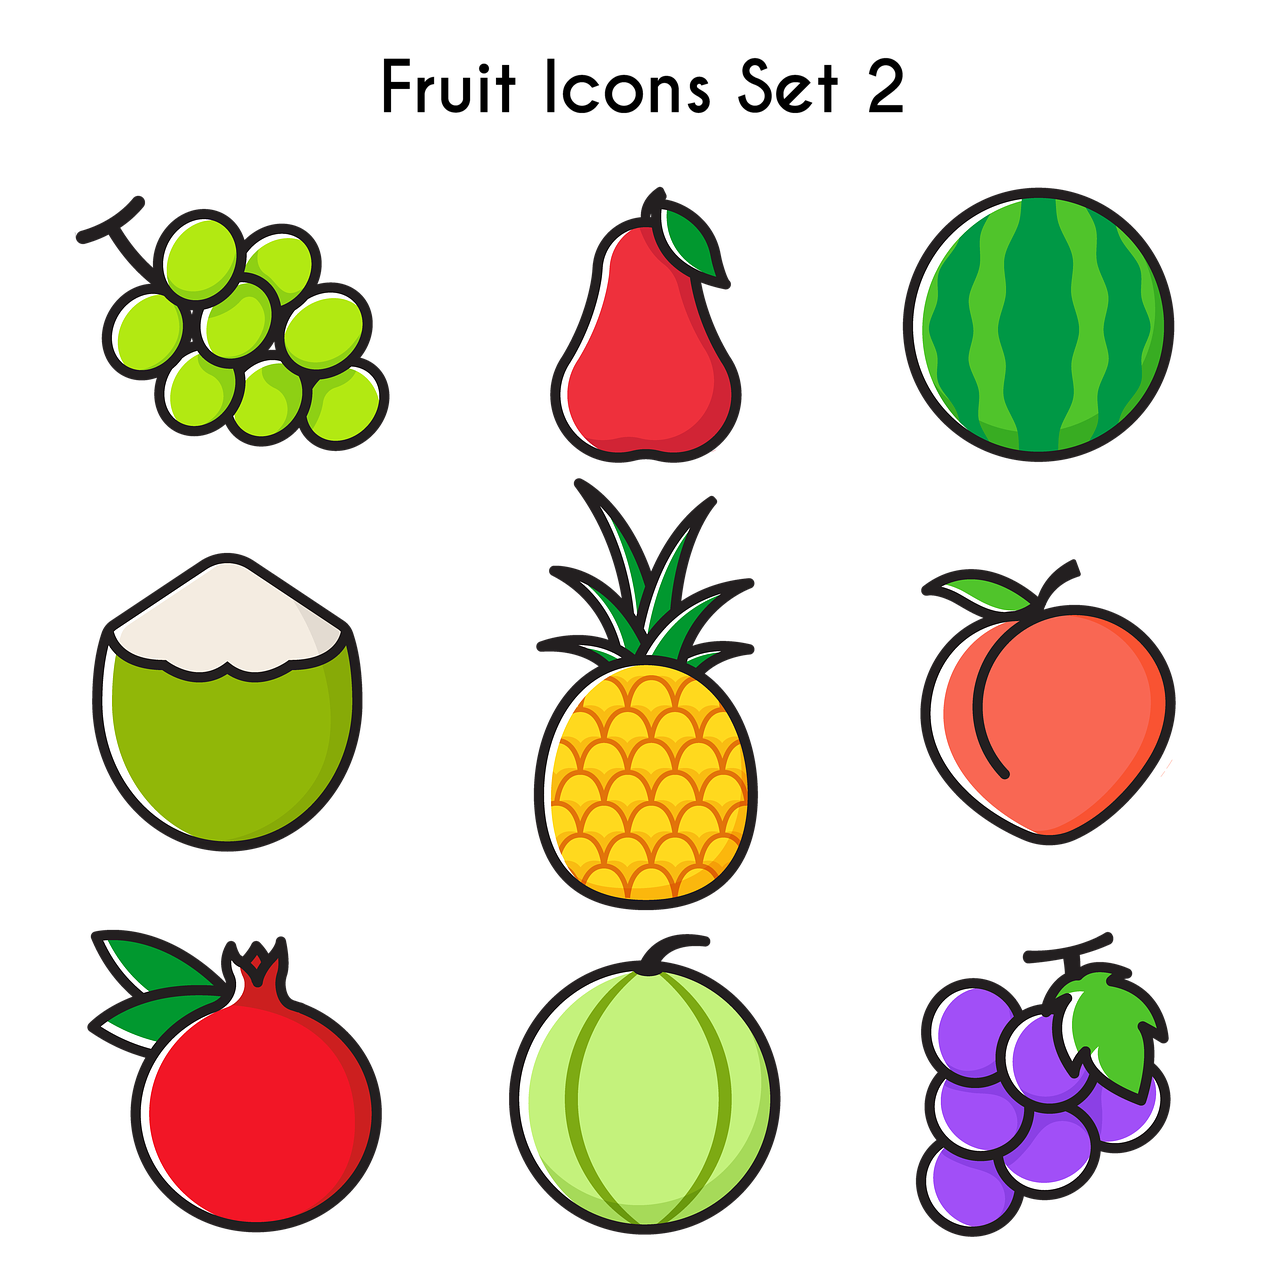
\includegraphics[width=\marginparwidth]{./images/PNLD2022-005-10.png}\\
Outro exemplo de imagem que pode ser utilizada na atividade de categorização de elementos. (Pixabay; CC-BY-2.0)}


%950 caracteres
\item \textbf{A atividade}\quad Prepare a sala para que o ambiente fique o mais livre possível para desenvolver a atividade. o professor deverá explicar para as crianças que elas poderão ir em duplas para pegar a imagem na caixa. Explique as categorias (plantas, animais e pessoas) e o que devem fazer quando a atividade iniciar. O professor deverá perguntar em qual das categorias abordadas a imagem que a criança (ou dupla) pegou se encaixa e estimulá-la a levar até a mesa com a categoria correspondente. É importante perguntar também se sabem com qual letra do alfabeto a imagem começa. Se não souberem procure fazer perguntas facilitadoras, mas, se mesmo assim os alunos não conseguirem, diga a letra. Repita o processo até que todos os alunos tenham participado.


%550 caracteres
\item \textbf{Interação}\quad O livro pode e deve ser 
manipulado pelos estudantes. Incentive que eles tentem repetir algum trecho dos poemas de que se recordam,
faça perguntas e proponha que imaginem juntos como é a vida 
de alguns dos animais explorados durante a leitura. Quando as crianças propuserem suas ideias, interaja com o pensado e apresentado pelas crianças, fazendo perguntas que as auxiliem a desenvolver o pensamento iniciado.
Relacione os animais sobre os quais falaram com as letras do alfabeto, mostrando a ordem das letras e fazendo perguntas como: ``com qual letra se inicia a palavra warima?'', ``onde está, na ordem do alfabeto, a letra W?''.

\item \textbf{Perguntas para avaliar}\quad Perguntas para avaliar: Os alunos conseguiram trabalhar em dupla? Se ajudaram? Realizaram o trabalho proposto? Como se posicionaram diante dos desafios? 
\end{enumerate}


\section{Literacia familiar}
O \textsc{pna} dá destaque especial para a importância do envolvimento da família 
no processo pedagógico nesta faixa etária e denomina Literacia Familiar o conjunto 
de experiências e práticas relacionadas à linguagem (oral, escrita ou lida) vivenciadas 
com os cuidadores. 

Essas estratégias podem começar a ser colocadas em prática desde a 
gestação e continuar até o final da adolescência. São práticas simples e divertidas 
que estimulam o desenvolvimento de quatro atividades fundamentais: ouvir, falar, 
ler e escrever que criam momentos de afeto e interação para a família. 

Para que esse trabalho conjunto entre escola e família funcione, é 
fundamental que a escola esteja em constante diálogo com os responsáveis e 
você consiga orientá-los. Um grupo em aplicativos de mensagens instantâneas ou um 
grupo de e-mails são saídas viáveis para que a comunicação se estabeleça e pode ser 
uma forma útil das famílias compartilharem suas vivências e trocarem sugestões 
de abordagens, sempre contando com a sua mediação. 

Com o objetivo de incentivar 
a prática da \textit{literacia familiar}, se possível, organize um rodízio entre os familiares 
das crianças para emprestar o livro da biblioteca da turma. Neste caso, crie um caderno 
de registro e estabeleça períodos para cada família ficar com o livro. É importante 
que os familiares compreendam a seriedade deste compromisso, pois o livro pertence 
ao acervo da sala e, portanto, deve ser bem cuidado e devolvido na data acordada. 

Se não for possível garantir o acesso direto dos cuidadores da criança ao livro, 
grave um vídeo direcionado a eles, contando a história e apresentando algumas 
das ilustrações. O importante é que os familiares saibam com clareza qual livro 
está sendo trabalhado, a história contada e se sinta seguro para explorar as temáticas 
do livro com a criança. Orientações claras e a manutenção do canal de comunicação com 
os responsáveis é essencial para que eles se sintam seguros e à vontade para fazer perguntas 
se tiverem dúvidas. 

Neste manual, você encontrará algumas práticas que podem ser 
recomendadas aos familiares para ajudá-los a expandir e aprofundar o trabalho 
que você iniciou em sala de aula.


\subsection{Importância da leitura}
Na escola, aprendemos a ler letras, mas é importante ter em mente que nós 
lemos o mundo desde muito pequenos: “lemos” os animais que passam pelos nossos 
quintais, a expressão no rosto dos nossos familiares, as cores que pintam o céu 
em um fim de tarde. 

Vamos aprendendo, ao longo da vida, a interpretar acontecimentos 
e sons que escutamos e a utilizá-los para nossa comunicação. Aprender a ler textos e 
escrevê-los expande a nossa leitura do mundo, pois permite que sejamos capazes de 
interpretar um código e experimentar, a partir dele, novas experiências e conhecimentos. 

O simples contato com os livros já permite um leque grande de sensações: 
sentimos as texturas, as formas, vemos as cores do livro, escutamos o som da página 
virando e o som da voz do narrador, se a história estiver sendo lida em voz alta. Para uma 
criança pequena, são experiências que podem contribuir diretamente com o desenvolvimento psicomotor 
e cognitivo. 

Nosso papel, enquanto mediadores de leitura, é contribuir para que essas 
sensações sejam associadas a momentos positivos, de construção de 
conhecimento e exercício de imaginação. 

Com os livros, podemos conhecer mais da história humana, descobrir informações 
novas sobre sociedades diferentes da nossa, imaginar situações e contextos inéditos 
para nós e aumentar o nosso repertório. São por meio deles que melhoramos nossa 
capacidade de interpretação, de expressão, de análise e senso crítico. Boas habilidades 
leitoras podem contribuir para o desenvolvimento de um estudante em todas as outras 
disciplinas, pois exercem influência direta na forma como absorvemos e 
construímos conhecimento.


\subsection{O papel da família na formação do leitor}
A família é peça fundamental na formação do leitor, pois é ela quem primeiro 
ensina a criança a ler. Não apenas os textos escritos, mas a ler o mundo, a 
interpretar os estímulos que a cercam, a construir seu próprio vocabulário e a 
comunicar seus pensamentos e necessidades.

O universo das letras é muito presente na vida das crianças antes mesmo de sua 
entrada na escola. Aparece nas histórias e ilustrações do livro que o cuidador 
lê ao colocá-la para dormir, nas situações em que vê os responsáveis se comunicarem 
pela escrita ou nos textos que podem permear seu cotidiano (nos outdoors, na 
televisão, no celular, manuais de instrução entre outros). 

Os familiares têm, 
portanto, uma ótima oportunidade de apresentar a leitura com leveza, de forma 
prazerosa, associado ao contexto em que a criança vive e à momentos de diversão. 
Você poderá orientar os pais nesta tarefa, ensinando-os com este guia a aproveitar 
as oportunidades para trabalhar a Literacia com a criança.


\subsubsection{Práticas de literacia familiar} 

São muitas as experiências que a prática da \textit{literacia familiar} 
pode oferecer às crianças. A seguir, explicamos cada uma delas para que você possa, 
se achar necessário, compartilhar com os responsáveis enquanto estiver orientando-os: 

\paragraph{Interação verbal} Aumentar a quantidade de conversas com as 
crianças, fazendo perguntas para incentivar o diálogo.

\paragraph{Leitura dialogada} Interagir com a criança durante a leitura 
em voz alta, criar expectativa sobre o livro, chamar a atenção para detalhes 
das ilustrações e comentar o enredo.

\paragraph{Narração de histórias} Interagir com a criança enquanto 
estiver narrando uma história, por exemplo, incluindo-a na ação, utilizando 
marionetes ou permitindo que ela complete a narrativa.

\paragraph{Contatos com a escrita} Apresentar as letras para as 
crianças, incentivar que tentem escrever ou ler, ajudá-los a desenhar letras, 
entre outras formas de incentivar o contato com as palavras.

\paragraph{Atividades diversas} Qualquer atividade com a criança 
pode ser utilizada para contribuir para a alfabetização. Jogos, brincadeiras, 
instrumentos musicais, canto, dança, passeios e viagens oferecem boas 
oportunidades de aprendizado.

\paragraph{Motivação} Atitudes que motivem as crianças à envolver-se com 
o mundo da leitura e da escrita.

\subsection{Exercitando a literacia familiar}

\BNCC{EI03EO04}
\BNCC{EI03EO06}
\BNCC{EI03CG02}
\BNCC{EI03ET01}
\BNCC{EI03ET05}

\begin{enumerate}
%700 caracteres
\item \textbf{Como começar}\quad O contato da família com a criança e o livro começam desde a primeira atividade proposta. Ao escolher objetos para levar para a escola com a letra do alfabeto designada para cada criança, os pais terão papel fundamental em auxiliar a escolha dos filhos em consonância com a proposta da atividade. Instrua os pais para que não escolham pelos filhos, mas reflitam com eles sobre objetos com as letras do alfabeto. Assim, as crianças vão começar a observar o alfabeto e suas letras em objetos cotidianos, apropriando-se gradualmente do sistema alfabético no ambiente doméstico. Instrua os pais em relação às figuras mobilizadas pelos poemas (os animais, as músicas, as lendas populares, as frutas etc.), de forma a que, em casa, também possam falar um pouco sobre esses elementos com as crianças.

%650 caracteres
\item \textbf{Leitura}\quad A família pode continuar 
explorando os temas apresentados pelo livro. Os familiares podem fazer isso ao relacionar 
elementos do cotidiano que aparecem na história e indicar a conexão 
entre o que viram na ilustração e a realidade. Peça para os pais estimularem o reconhecimento das letras mostrando revistas, letreiros nas ruas, frases escritas em roupas, orientando para que, no cotidiano, seja trabalhado o conteúdo do livro, facilitando assim a generalização do conhecimento. A pesquisa dos animais e outros elementos desconhecidos no poema também pode ser realizada em casa com a ajuda dos familiares, dentro das possibilidades concretas de cada família. Outra possibilidade, quando a família tem acesso ao livro, é ler alguns poemas com a criança em um horário estipulado para isso. A leitura em família é importante pois relaciona o ato de ler e manusear um livro com o campo de suas experiências afetivas.

%1073 caracteres
\item \textbf{Instrução}\quad Informe aos pais sobre a estrutura do livro e as principais competências desenvolvidas em sala de aula, ressaltando a importância de seguir as letras do alfabeto em sua relação com os elementos (textuais e imagéticos) que remetem a diferentes culturas e regiões do Brasil.
Oriente-os a, quando possível, ler algum dos poemas com a criança.
Desta forma as crianças terão contato com a mesma história de duas formas distintas, através da mediação em sala de aula e em família. 
Mesmo pequenas, as crianças conseguem perceber a diferença entre 
as formas de contar, e elementos da narração em casa podem ajudá-la a compreender 
sentidos e perceber detalhes que não foram explorados em sala de aula. Se possível, depois da leitura, oriente 
que voltem ao livro e tentem identificar as letras dos nomes de animais, figuras folclóricas etc. com o apoio das  ilustrações. 

Outra opção é entregar o livro para a criança e pedir que ela tente se lembrar
do que foi falado em sala de aula, quais elementos foram destacados e enfatizados pelo educador e pelos colegas. Mesmo que a memória não pareça 
completa para o adulto, é importante que ele ouça com atenção e 
valorize todas as tentativas da criança. Afinal, ao tentar recontar, 
ela manipulará o livro, treinará a coordenação motora, conhecerá as texturas 
do objeto e poderá imitar a forma como o adulto 
conta a história, treinando a fala. 

Também pode ser indicado para os pais músicas infantis com o abecedário, que podem ser escutadas em casa, e trabalha a memorização do alfabeto, reforçando a linguagem e o vínculo familiar. 
\end{enumerate}

 
\section{Sugestões de referências complementares}

\subsection{Livros} 

\begin{itemize}
\item \textsc{lins}, Guto. \textit{Livro infantil? projeto gráfico, metodologia, subjetividade}. São Paulo: Rosari, 2002.

Livro que aborda a importância das escolhas visuais (ilustração, projeto gráfico, lettering) na literatura infantil.  

\item \textsc{hunt}, Peter. \textit{Crítica, teoria e literatura infantil}. São Paulo: Cosac Naify, 2010.

Livro sobre crítica de literatura infantil que contêm definições de livro ilustrado e livro imagem. 
\end{itemize}

\subsection{Artigos}

\begin{itemize}
\item \textsc{sardelich}, Maria Emilia. Leitura de Imagens, Cultura Visual e Prática Educativa. 
In: Cadernos de Pesquisa. V.36, n.128, p.451-472, mai/ago.2006. Disponível em: \url{https://www.scielo.br/pdf/cp/v36n128/v36n128a09}. 
Acesso em 29 abr 2021. 

Artigo acadêmico que discorre sobre a importância de trabalhar cultura 
visual na educação na sociedade contemporânea. 

\item \textsc{pranke}, Marha Elfrida. Organização dos espaços da sala de aula na Educação Infantil. Disponível em: \url{http://centraldeinteligenciaacademica.blogspot.com/2016/04/organizacao-dos-espacos-da-sala-de-aula.html}. Acesso em 04 mai 2021. 

Artigo acadêmico que discorre sobre a importância da rotina e de criar ambientes dentro da sala de aula na Educação Infantil.  
\end{itemize}

\subsection{\textit{Sites}}

\begin{itemize}
\item Vídeos “Conta pra mim” no site do PNA. Disponível em: \url{http://alfabetizacao.mec.gov.br/contapramim}. 
Acesso em 13 abr. de 2021.

Página do \textsc{mec} com vídeos sobre leitura dialogada que visam incentivar a Literacia Familiar. Muitas das 
técnicas, explicações e materiais disponíveis nessa página podem ser utilizados em aula, mas o site também 
pode ser uma ótima indicação para ajudar a direcionar os cuidadores dos estudantes a praticar 
a literacia familiar e leitura dialogada.

\item Vídeo “Livros de imagem: como utilizar com as crianças?” do canal Conta Outra. Disponível em Youtube. 
Acesso em 14 abr. 2021. 

Neste vídeo, a pedagoga Bel explica o que são livros de imagem e faz sugestões para mediar a leitura com 
crianças. Se você achar conveniente, esse vídeo pode ser recomendado aos familiares da criança 
para inspirá-los na leitura dialogada. 
\end{itemize}

\section{Bibliografia comentada}

\subsection{Livros}

\begin{itemize}
\item \textsc{brasil}. Ministério da Educação. Base Nacional Comum Curricular. Brasília, 2018.

Consultar a \textsc{bncc} é essencial para criar atividades para a turma. Além de especificar 
quais habilidades precisam ser desenvolvidas em cada ano, é fonte de informações sobre 
o processo de aprendizagem infantil. 

\item \textsc{brasil}. Ministério da Educação. Secretaria de Alfabetização. Conta pra mim: Guia de Literacia Familiar. 
Brasília: \textsc{mec, sealf}, 2019. Disponível em: \url{http://alfabetizacao.mec.gov.br/images/conta-pra-mim/conta-pra-mim-literacia.pdf}.

Este guia é voltado aos pais e oferece explicações em uma linguagem bastante acessível e detalhada as práticas de Literacia Familiar, 
como praticar leitura dialogada, como narrar histórias, como exercitar interação oral, formas de proporcionar contatos com a escrita à criança etc. 
 
\item \textsc{brasil}. Ministério da Educação. Secretaria de Alfabetização. PNA Política Nacional de Alfabetização/Secretaria 
de Alfabetização. Brasília: \textsc{mec, sealf}, 2019.

Um guia fundamental para trabalhar pré-alfabetização e alfabetização de estudantes, que ressalta a importância da Literacia e da Numeracia. 

\item \textsc{van der linden}, Sophie. Para ler o livro ilustrado. São Paulo: Cosac Naify, 2011.

Livro sobre as particularidades do livro ilustrado, que apresenta as diferenças entre o livro ilustrado e o livro com ilustração. 
\end{itemize}

\subsection{Artigos}

\begin{itemize}
\item \textsc{costa}, A. C. C.; \textsc{santos neto}, J. A.; \textsc{bortolin}, S; \textsc{pereira}, Ana Paula. O livro de imagem e a mediação na escola. 
In \textsc{vii secin}, Universidade de Londrina. Disponível em \url{http://www.uel.br/eventos/cinf/index.php/secin2017/secin2107/paper/viewFile/445/296}. 
Acesso em 29 abr 2021
. 
Esse artigo reflete sobre a importância de se apresentar livros de imagem para os estudantes na escola para que as crianças aprendam a ler imagens. 

\item \textsc{nannini}, P. B. R.; \textsc{medeiros}, J. P. S.; \textsc{ribeiro}, J. M. Leitura em cena: Vivências em sala de aula com livro de imagens. 
Literartes, n. 3, p. 82-101, 2014. DOI: 10.11606/issn.2316-9826.literartes.2014.89204. 
Disponível em \url{https://www.revistas.usp.br/literartes/article/view/89204/92115}. Acesso em 29 abr. 2021. 

Artigo acadêmico sobre um trabalho utilizando o mesmo livro de imagem com crianças da educação infantil e ensino médio. 
É uma forma interessante de perceber que a leitura de imagens pode ser explorada com qualquer faixa etária. 
\end{itemize}

% 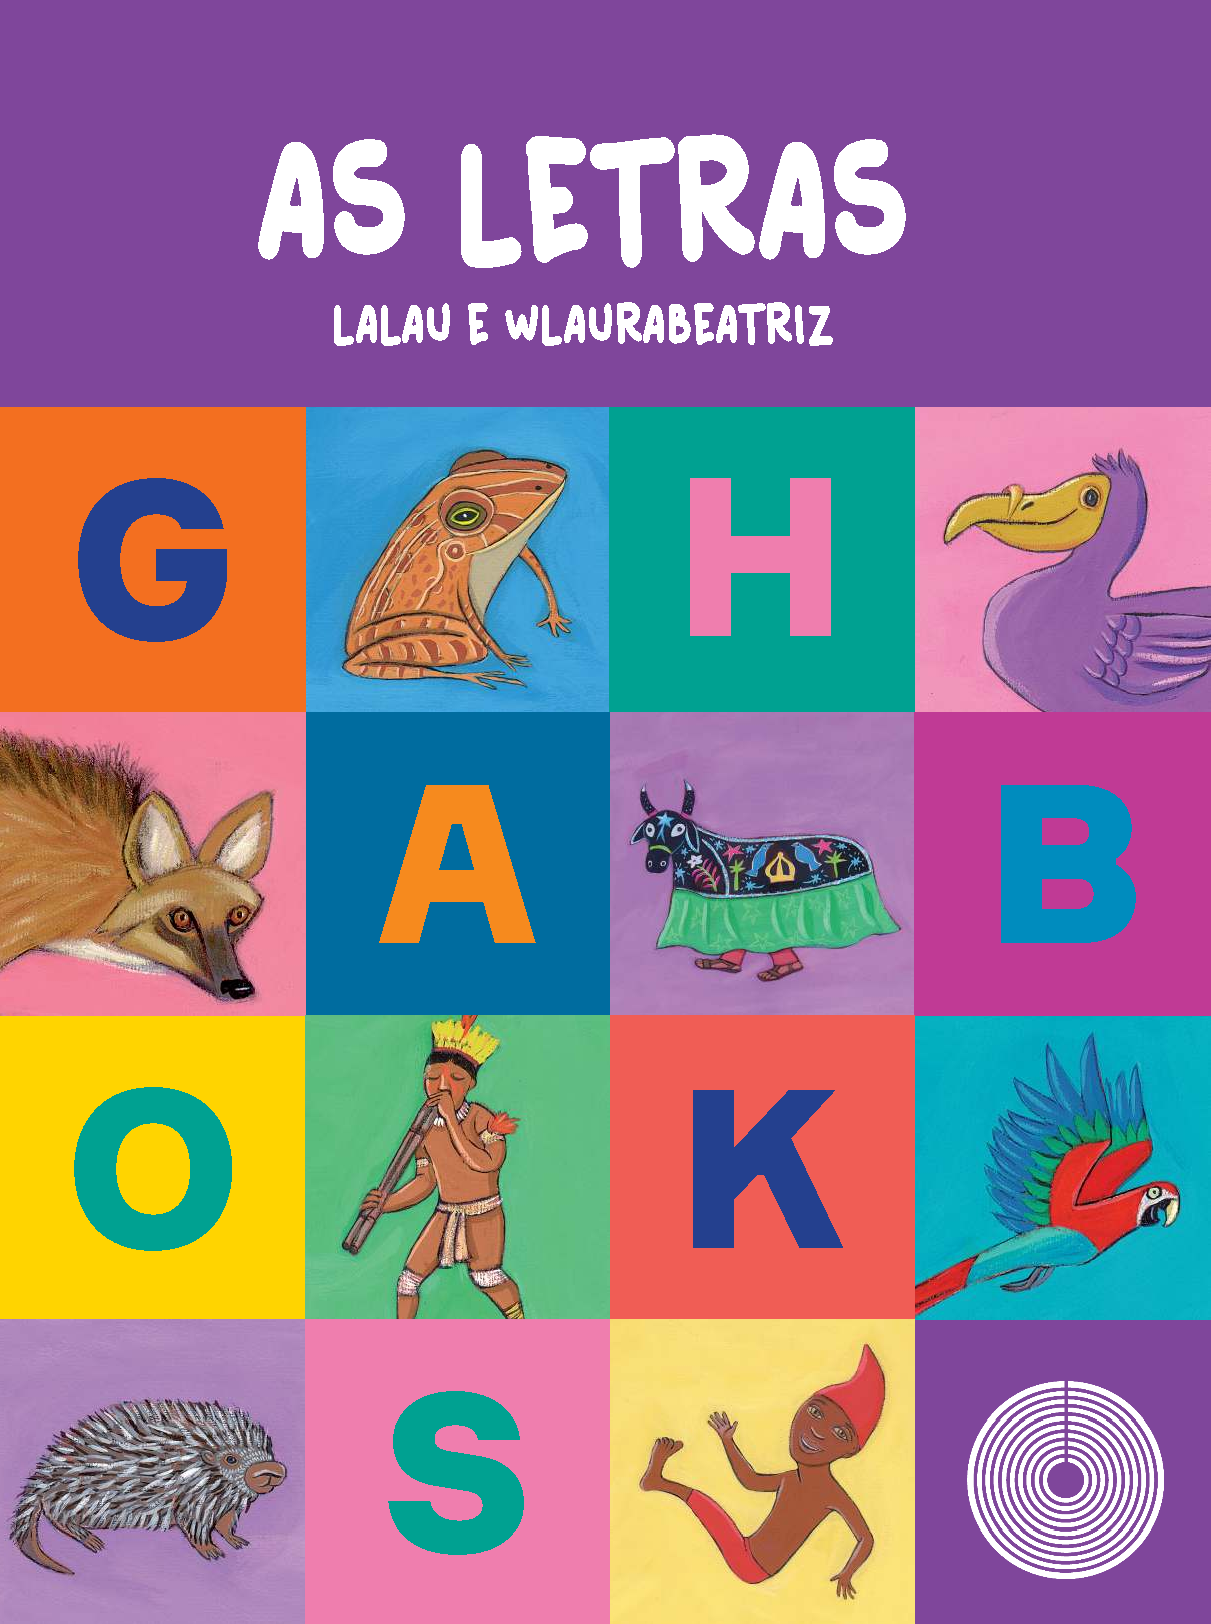
\includepdf[nup=2x2, 					% grid
			% offset=-15mm -5mm, 		% posição
			% scale=.8, 				% tamanho da página
            % delta=4mm 4mm, 			
            % frame,
            % pages={1-4}]{pdfs/PNLD2022-005_MIOLO.pdf}

\end{document}
